\documentclass{article}
\usepackage{graphicx} % Required for inserting images
\usepackage{amssymb}
\usepackage[margin=3cm]{geometry}
\usepackage{amsmath}
\usepackage{amsthm}
\usepackage{enumitem}
\usepackage{accents}
\usepackage{wasysym}
\usepackage{hyperref}
\usepackage{mdframed}

\renewcommand{\contentsname}{Índice de Contenidos}

\begin{document}

\begin{titlepage}
    \begin{center}
        {\Huge \textsc{Ecuaciones Diferenciales \\ \vspace{10px} Ordinarias}}
    \end{center}

    \vspace{10px}

    \hfill{\textit{-- Alto, policía, a cometido usted un crimen.}}

    \hfill{\textit{-- Lo asumo.}}

    \hfill{\textit{-- Lo arresto.}}

    \tableofcontents
\end{titlepage}

\newpage

\section{Soluciones Ejercicios}

En esta sección se detallarán los argumentos utilizados para resolver los ejercicios planteados en clase (una selección de ellos, que me canso).

\subsection{Relación 1}
\label{seq:1:1}

\begin{enumerate}
    \item \textit{Considera la EDO}
    
    \[x'(t) = x(t), \hspace{20px} t \in I \subset \mathbb{R}.\]

    \begin{itemize}
        \item \textit{Probar que si $x(t_0) = 0$ para algún $t_0 \in I$, entonces $x(t) = 0$ para todo $t \in I$.}

        \vspace{7px}

        \textsc{Demostración:} Supongamos, por reducción al absurdo, que existe $t_1 \in I$ tal que $x(t_1) \neq 0$. Además, no es ninguna pérdida de generalidad suponer que $x(t_1) > 0$.
        De esta información obtenemos inmediatamente que $t_0 < t_1$, pues apartir de $t_1$ la función es creciente. Más aún, podemos asumir sin miramientos que $t_0 = \max\{t \in I: x(t) = 0\}\footnote{Afirmar la existencia de dicho máximo se deja al ingenio del lector.}$ y que $t_1 - t_0 < 1$.

        Después de establecer estas hipótesis y aclaraciones, lo primero que hacemos es aplicar el Teorema del Valor Medio para obtener que

        \[\frac{x(t_1) - x(t_0)}{t_1 - t_0} = x'(t_2), \hspace{20px} t_2 \in (t_0, t_1),\]

        de donde sacamos

        \[x(t_1) = x(t_2)(t_1 - t_0)\]

        usando la condición de la EDO propuesta.

        Repitiendo este proceso de manera reiterada, podemos construir una sucesión $(t_n)_n \subset I$ tal que, para cada $n \geq 2$, $t_n$ es un punto del intervalo $(t_0, t_{n-1})$ que satisface

        \[x(t_{n-1}) = x(t_n)(t_{n-1} - t_0).\]

        Mediante una supérflua inducción se puede argumentar fácilmente que, considerando la sucesión

        \[a_n = x(t_n)(t_{n-1} - t_0)(t_{n-2} - t_0) \dots (t_1 - t_0),\]

        se tiene que $x(t_1) = a_n$ para todo $n \in \mathbb{N}$, por lo que $\lim_{n \to \infty} (a_n) = x(t_1)$. No obstante, por otra parte, es fácil notar a partir de las hipótesis marcadas que $a_n \leq x(t_1)(t_1 - t_0)^{n-1}$ y, en consecuencia, como $t_1 - t_0 < 1$, que $\lim_{n \to \infty} (a_n) = 0$. En definitiva, hemos inferido que $x(t_1) = 0$, lo cual contradice la suposición inicial de que $x(t_1) > 0$, por lo que concluimos que $x$ debe ser nula en todo $I$. \hfill{\textsc{Q.e.d.}}

        \vspace{7px}

        \item \textit{Sean $x(t), y(t)$ soluciones de la EDO con $y(t) \neq 0$. Probar que existe $\lambda \in \mathbb{R}$ tal que $x(t) = \lambda y(t)$.}
        
        \vspace{7px}

        \textsc{Demostración:} Sea $\lambda : I \longrightarrow \mathbb{R}$ una función tal que $\lambda(t) = x(t)/y(t)$ para todo $t \in I$, función la cual está bien definida debido a que $y(t) \neq 0$ en todo su dominio (apartado anterior).

        A continuación, si derivamos, obtenemos que

        \[\lambda'(t) = \frac{x'(t)y(t) - x(t)y'(t)}{(y(t))^2},\]

        y, usando la información sobre la EDO, nos queda que

        \[\frac{x'(t)y(t) - x(t)y'(t)}{(y(t))^2} = \frac{x(t)y(t) - x(t)y(t)}{(y(t))^2} = 0,\]

        por lo que $\lambda'(t) = 0$ y, por subsiguiente, la función $\lambda(t)$ es constante. Llamemos $\lambda \in \mathbb{R}$ a dicha constante\footnote{Abuso de lenguaje o si como me gusta caramba.}.

        Por cómo habíamos construido la función es inmediato observar que $x(t) = \lambda y(t)$, que es lo que tanto ansiábamos. \hfill{\textsc{Q.e.d.}}

        \vspace{7px}

        \item \textit{Concluir que las únicas soluciones de esta EDO son de la forma $x(t) = \lambda e^t, \lambda \in \mathbb{R}$.}
        
        \vspace{7px}

        \textsc{Solución:} Es un resultado inmediato invocando el apartado anterior, ya que la función $y(t) = e^t$ satisface la EDO del ejercicio. $\hfill\square$
    \end{itemize}

    \vspace{12px}

    \item \textit{Probar que si $x(t)$ es una solución de la EDO}

    \[x''(t) + x(t) = 0,\]

    \textit{entonces es también solución de}

    \[x'(t)^2 + x(t)^2 = k,\]

    \textit{para algún $k \in \mathbb{R}$.}

    \vspace{7px}

    \textsc{Demostración:} Aunque no se especifica en el enunciado, 
    suponemos que el dominio de definición de $x$ es todo $\mathbb{R}$. Habiendo hecho esta puntualización inicial, comenzamos suponiendo que $x''(t) + x(t) = 0$. A continuación, consideramos $f : \mathbb{R} \longrightarrow \mathbb{R}$ tal que 
    
    \[f(t) = x'(t)^2 + x(t)^2, \hspace{20px} \forall t \in \mathbb{R}.\]

    Al tomar la derivada de $f$ notamos que

    \[f'(t) = 2x'(t)x''(t) + 2x(t)x'(t) = 2x'(t)(x''(t) + x(t)),\]

    y, aplicando la hipótesis, llegamos a que

    \[2x'(t)(x''(t) + x(t)) = 2x'(t) \cdot 0 = 0,\]

    por lo que sabemos que $x'(t)^2 + x(t)^2 = f(t) = k$ para todo $t$ real, donde $k \in \mathbb{R}$ es una constante. Este hecho es consecuencia de que la derivada sea nula en todo su dominio. \hfill{\textsc{Q.e.d.}}

    \vspace{7px}

    \textit{Encontrar una solución de $x'(t)^2 + x(t)^2 = k$ que no sea solución de $x''(t) + x(t) = 0$.}

    \vspace{7px}

    \textsc{Solución:} Para cualquier $k > 0$ tomamos la función $x(t) = \sqrt{k}$, donde notamos inmediatamente que satisface $x'(t)^2 + x(t)^2 = k$, mientras que obviamente no es solución de la otra. $\hfill\square$

    \newpage

    \textit{¿Qué tiene que cumplir una solución de $x'(t)^2 + x(t)^2 = k$ para ser solución de $x''(t) + x(t) = 0$?}

    \vspace{7px}

    \textsc{Solución:} Descartamos el caso $k = 0$ pues en ese se cumplen ambas EDOs trivialmente, por lo que de ahora en adelante asumiremos $k > 0$. Ahora si, en primer lugar, se tiene que cumplir que $x \in C^2$ para poder considerarla solución de la segunda EDO. Además, vamos a probar que otra condición necesaria\footnote{Esta condición de hecho también es suficiente, pero se sale de los contenidos de este curso.} que tiene
    que satisfacer es que, considerando $D := \{t \in \mathbb{R}: x'(t) \neq 0\}$, se debe tener $D$ denso en $\mathbb{R}$.

    Para probar que es una condición necesaria, supongamos que $D$ no es denso en $\mathbb{R}$ y veamos que no es solución de la segunda EDO. 
    
    En consecuencia, como $D$ no es denso en $\mathbb{R}$, $\overline{D} \neq \mathbb{R}$ o, lo que es lo mismo, existen $t_0, r \in \mathbb{R}$ tales que $(t_0 - r, t_0 + r) \cap D = \emptyset$. Por tanto, para todo $t \in (t_0 - r, t_0 + r)$
    se tiene $x'(t) = 0$, con lo que deducimos que $x$ es constante en dicho intervalo.

    Al ser constante, y sabiendo que $x'(t)^2 + x(t)^2 = k$ con $x'(t) = 0$, obtenemos que $x(t) = \sqrt{k} > 0$ en todo el intervalo\footnote{También podría tomar la solución negativa $-\sqrt{k}$, pero no afecta al argumento.}. Con esta información llegamos fácilmente a que no satisface $x''(t) + x(t) = 0$,
    pues $x''(t) = 0$ mientras que $x(t) > 0$. $\hfill\square$

    \vspace{12px}

    \item \textit{Se considera el problema de Cauchy}
    
    \[
    \begin{cases}
        x'(t)^2 + x(t)^2 = a^2, \\
        x(0) = b.
    \end{cases}
    \hspace{20px} a \geq 0, b \in \mathbb{R}.
    \]

    \begin{itemize}
        \item \textit{Probar que $x(t) = a\sin t$ es solución de la EDO.}
        
        \vspace{7px}

        \textsc{Demostración:} Es un proceso desmesuradamente metódico, pero habrá que redactar o 
        el referí se queja. El primer paso (y prácticamente el último) es calcular la derivada

        \[x'(t) = a\cos t,\]

        con lo que ya obtenemos que

        \[x'(t)^2 + x(t)^2 = a^2\cos^2t + a^2\sin^2t = a^2(\cos^2t + \sin^2t) = a^2.\]

        \hfill{\textsc{Q.e.d.}}

        \vspace{7px}

        \item \textit{Probar que si $a < |b|$ entonces el problema anterior no tiene solución.}

        \vspace{7px}

        \textsc{Demostración:} Vamos sin rodeos. Como $x'(t)^2 \geq 0$, entonces nos queda que 

        \[x(t)^2 \leq x'(t)^2 + x(t)^2 = a^2,\]

        de donde sacamos que $x(t) \leq a$ y, en particular, $x(0) \leq a < |b|$, por lo que concluimos que no se puede dar $x(0) = b$. \hfill{\textsc{Q.e.d.}}

        \vspace{7px}

        \newpage

        \item \textit{Usando que $x(t) = a\sin t$ es una solución de la EDO, encontrar una solución del problema de Cauchy cuando $|b| \leq a$.}

        \vspace{7px}

        \textsc{Solución:} En primer lugar, como $|b| \leq a$, llegamos a que\footnote{Hemos descartado implícitamente el caso $a = 0$, pues no aporta ningún interés.}

        \[|b| \leq a \Longrightarrow -a \leq b \leq a \Longrightarrow -1 \leq \frac{b}{a} \leq 1,\]

        con lo que se deduce que existe $t_0 \in \mathbb{R}$ tal que $\sin t_0 = b/a$. Apartir de aquí el ejercicio se escribe solo,
        basta tomar la función $x(t) = a\sin(t + t_0)$ y ver que cumple las condiciones del problema de Cauchy planteado. En efecto,
        comprobar que verfica la EDO se lleva a cabo de una manera análoga al primer apartado, y en cuanto a la condición inicial, se reduce 
        simplemente a desarrollar

        \[x(0) = a\sin(0 + t_0) = a \cdot \frac{b}{a} = b.\]

        $\hfill\square$
    \end{itemize}

    \item \textit{Reducir las siguientes EDOs de segundo orden a un sistema equivalente de primer orden}
        
    \[a) \hspace{10px} x''(t) = \frac{1 - x'(t)^2}{x(t)} - 2k\sqrt{1 - x'(t)^2}, \hspace{15px} b) \hspace{10px} x''(t) = f(x'(t))x(t),\]

    \[c) \hspace{10px} \sin x'''(t) + \cos x''(t) + \tan x'(t) = x^2(t) - 1. \hspace{88px}\]

    \vspace{7px}

    \textsc{Solución:} To be continued.

    \vspace{12px}

    \item \textit{Se define}
    
    \[x(t) = x(t_0) + \int_{t_0}^{t} tf(s, x(s))\, ds,\]

    \textit{siendo $f$ una función continua. ¿Qué EDO cumple $x(t)$?}

    \vspace{7px}

    \textsc{Solución:} En primer lugar, notamos que

    \[\int_{t_0}^{t} tf(s, x(s))\, ds = t \int_{t_0}^{t} f(s, x(s))\, ds,\]

    para que, a lo hora de derivar, obtener

    \[x'(t) = \int_{t_0}^{t} f(s, x(s))\, ds + tf(t, x(t)).\]

    Además, si ``despejamos'' de la ecuación original la expresión $\int_{t_0}^{t} f(s, x(s))\, ds$ concluimos el ejercicio con la EDO en forma normal\footnote{La seguridad sobre esta afirmación va menguando cada vez más.}

    \[x'(t) = \frac{x(t) - x(t_0)}{t} + tf(t, x(t)).\]

    $\hfill\square$

    \newpage

    \item \textit{Encontrar una EDO que admita como soluciones a las siguientes familias de funciones.}

    \[a) \hspace{10px} x(t) = Ae^t + Be^{-t}, \hspace{20px} b) \hspace{10px} x(t) = Ae^t + Bte^t, \hspace{20px} c) \hspace{10px} x(t) = Ae^t\cos t + Be^t\sin t.\]

    \vspace{7px}

    \textsc{Solución:} Contestemos ordenadamente a los distintos apartados.

    \begin{itemize}
        \item[$a)$] En este caso es fácil deducir que una EDO que cumple la solicitud del enunciado se trata de
        
        \[x''(t) = x(t),\]

        de donde la inspiración puede provenir de las funciones trigonométricas hiperbólicas.

        \item[$b)$] En este caso hay que estrujar algo más los sesos. Primero calculamos la primera derivada, quedándose
        
        \[x'(t) = Ae^t + Bte^t + Be^t = x(t) + Be^t,\]

        de donde se deduce que $Be^t = x'(t) - x(t)$. A continuación, calculamos la segunda derivada

        \[x''(t) = Ae^t + Bte^t + 2Be^t = x(t) + 2(x'(t) - x(t)),\]

        a paritr de lo cual concluimos sin mucho esfuerzo que la EDO satisfecha por esta familia es

        \[x''(t)  = 2x'(t) - x(t).\]

        \item[$c)$] Me aburro, se deja como enigma al cuidado del lector\footnote{Indicación: deriva, anda.}.
    \end{itemize}

    $\hfill\square$

    \vspace{12px}

    \item \textit{Se considera la EDO}
    
    \[x'(t) = t + x(t)^3.\]

    \textit{Se pide:}

    \begin{itemize}
        \item \textit{Representar de forma aproximada las isoclinas.}

        \vspace{7px}

        \textsc{Solución:} Usar el comando \texttt{plot2d} en \textit{wxMaxima}. La representación gráfica de las curvas para $\lambda = -5, ..., 5$ es

        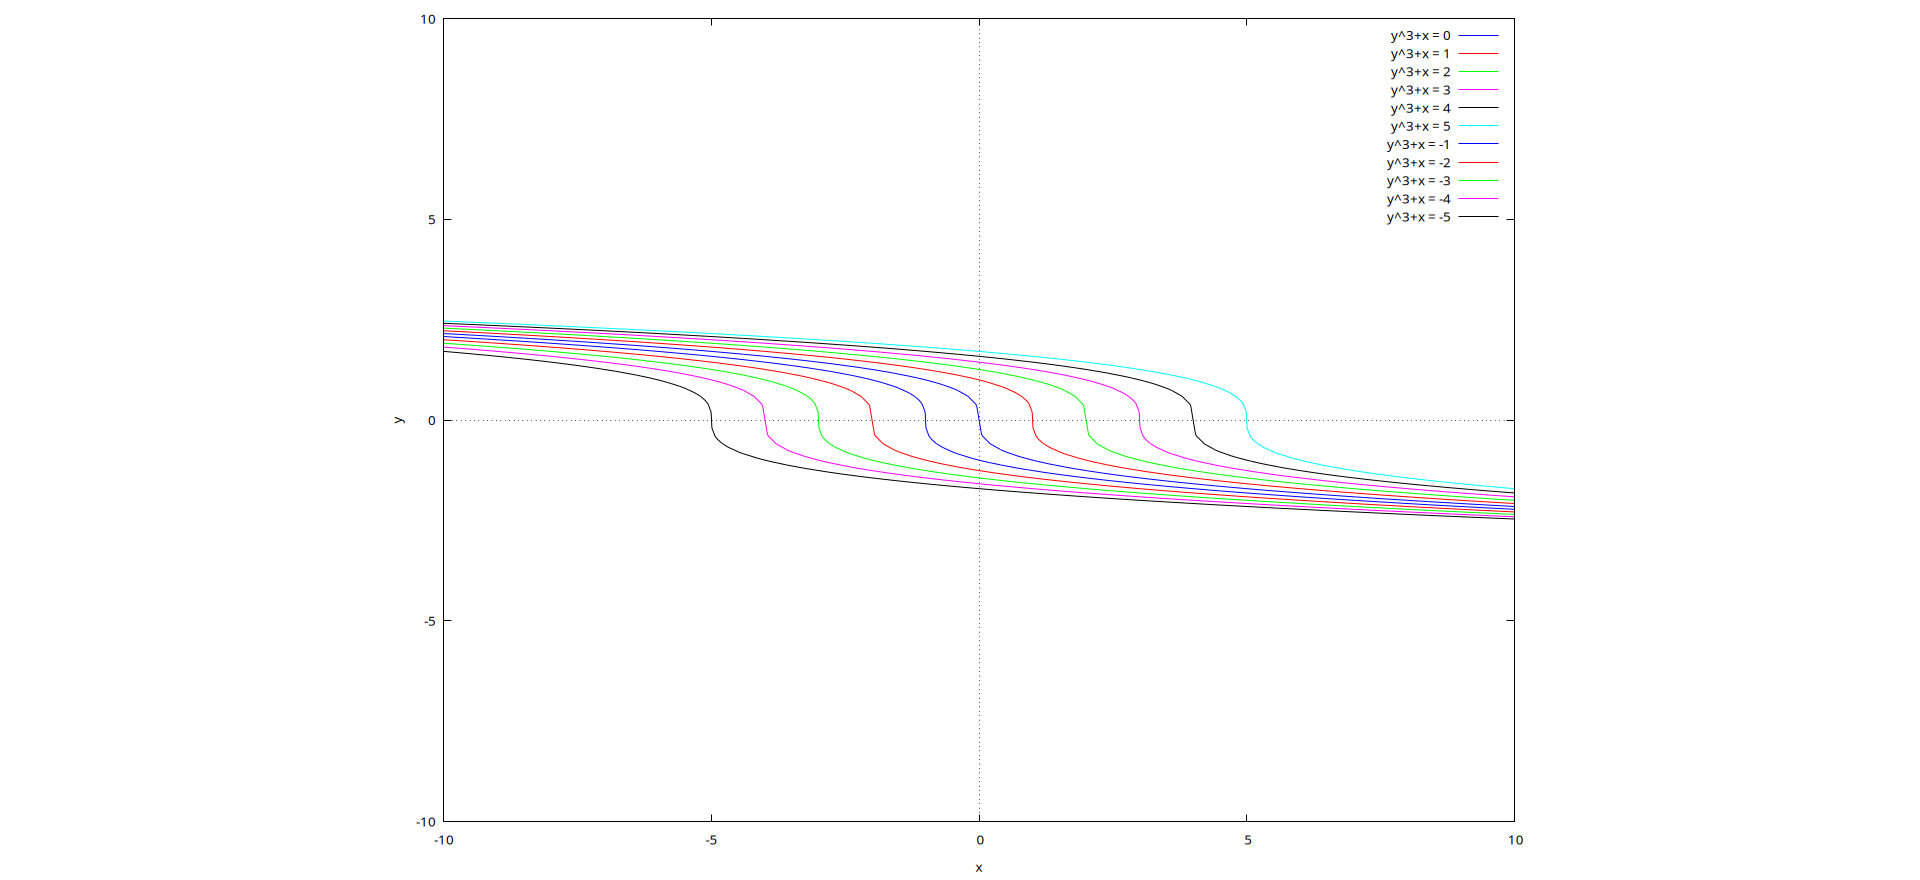
\includegraphics[width=\textwidth]{curva.png}

        $\hfill\square$

        \vspace{7px}

        \item \textit{Representar la curva en $\mathbb{R}^2$ donde las soluciones de la EDO alcanzan un punto crítico.}

        \vspace{7px}

        \textsc{Solución:} Se correspondería con la cruva generada al sustituir $\lambda = 0$. La ecuación que la representa es $x = \sqrt[3]{-t}$.

        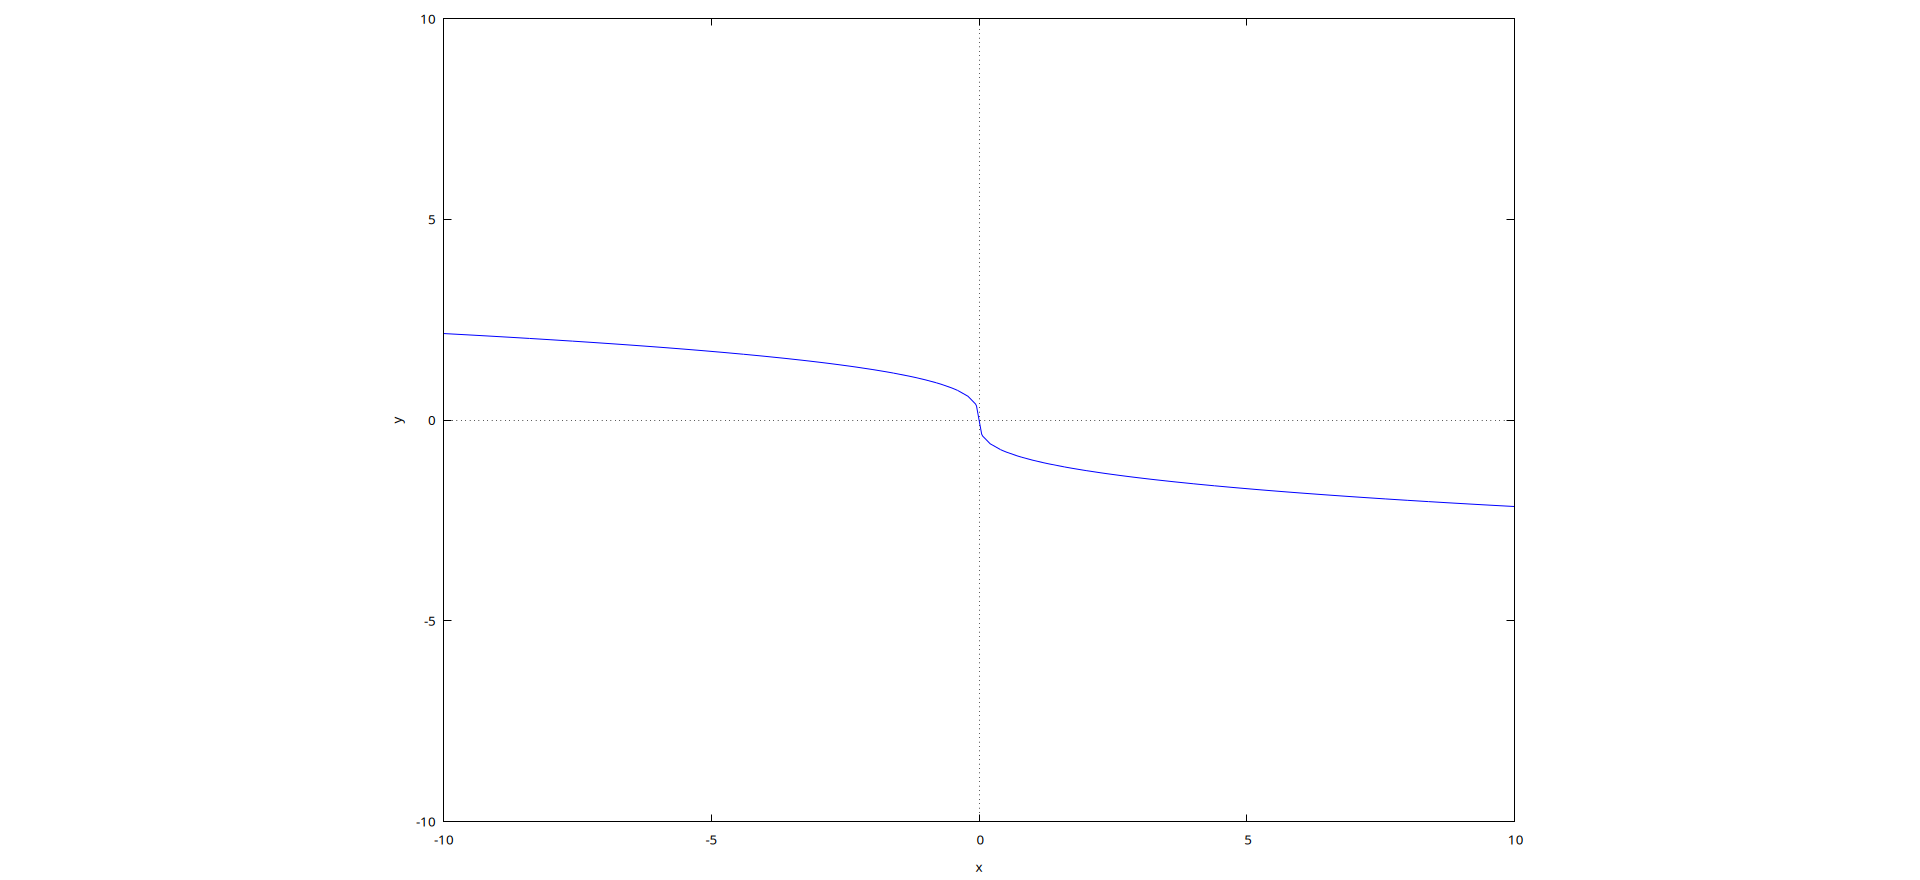
\includegraphics[width=\textwidth]{critico.png}

        $\hfill\square$

        \newpage

        \vspace{7px}

        \item \textit{Estudiar el número de ceros de una solución $x(t)$ en función de la condición inicial \\ $x(0) = x_0$.}

        \vspace{7px}

        \textsc{Solución:} Antes de comenzar a diferenciar entre los distintos casos, asentamos ciertas propiedades. Primero de todo, notamos que si la solución se encuentra por debajo de la curva del apartado anterior, entonces será decreciente, mientras que si se sitúa por encima será creciente. En segundo lugar, usando esta información, notamos que si una solución corta a la curva $x = \sqrt[3]{-t}$, entonces solo lo hará esa vez, por lo que esa intersección representa el único punto crítico de $x(t)$, que es de hecho mínimo absoluto (quizás convenga reflexionar esta afirmación). Con estas clarificaciones, hagamos el estudio pertinente:

        \begin{itemize}
            \item[($x_0 > 0$)] En este caso, la solución $x(t)$ no tendría ningún cero. Es sencillo ver que esto se debe a que el punto de corte con la curva de puntos críticos tiene lugar cuando $t < 0$, sección en la cual $\sqrt[3]{-t} > 0$, por lo que el mínimo de $x(t)$ será positivo y, en particular, distinto de 0.

            \item[($x_0 = 0$)] Se trata del caso más trivial, pues el mínimo absoluto se encuentra justamente en ese punto $t = 0$. To sum up, tiene un único 0.

            \item[($x_0 < 0$)] Por contra, este caso requiere de más detenimiento y racionalización, pues puede darse el caso en el que tenga uno o dos ceros. Lo cierto es que como se vio en clase me da soberano palo seguir redactando.
        \end{itemize}

        $\hfill\square$
    \end{itemize}

    \vspace{12px}

    \item \textit{Dada la curva}
    
    \[C = \{(t, x) \in \mathbb{R}^2 : t^2 + 2x^2 + 2t + 2x = 1\},\]

    \textit{se pide:}

    \begin{itemize}
        \item \textit{Estudiar cuántas componentes de $C$ se pueden extraer que se puedan expresar como un grafo $(t, x(t))$.}

        \vspace{7px}

        \textsc{Solución:} Aunque no es necesario, puede ser de utilidad darse cuenta de que $C$ se corresponde con una elipse. En concreto, viene descrita por la siguiente ecuación

        \[\left(\frac{t+1}{\sqrt{5/2}}\right)^2 + \left(\frac{x+1/2}{\sqrt{5}/2}\right)^2 = 1.\]

        Su representación gráfica sería la siguiente:

        \begin{figure}[h]
            \centering
            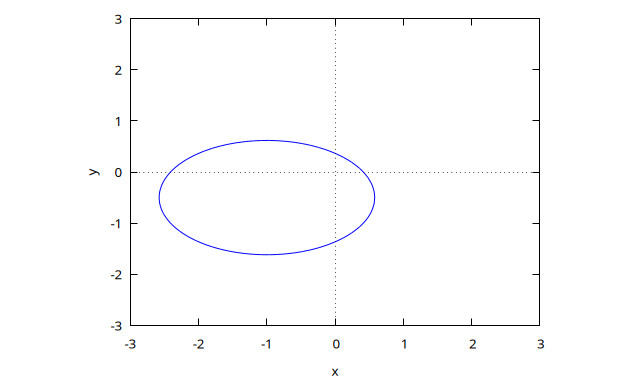
\includegraphics[width=200px]{eclipse.png}            
        \end{figure}

        Habiendo hecho este análisis previo es trivial notar que podemos separar la curva en dos grafos: la parte de ``arriba''; y la parte de ``abajo''. 
        Para obtener las expresiones explícitas podemos usar la fórmula de Bhaskara, de donde $x(t)$ para la parte superior es 

        \[x(t) = -\frac{1}{2} + \frac{\sqrt{-2t^2-4t+3}}{2},\]

        y para la parte inferior

        \[x(t) = -\frac{1}{2} - \frac{\sqrt{-2t^2-4t+3}}{2}.\]

        $\hfill\square$

        \vspace{7px}

        \item \textit{Encontrar una EDO de la forma $x'(t) = f(t, x(t))$ que admita como soluciones las funciones del apartado anterior.}

        \vspace{7px}

        \textsc{Solución:} Derivando se puede llegar sin muchos obstáculos a que una EDO que cumple las condiciones del enunciado es

        \[x'(t) = -\frac{t+1}{2x(t) + 1}.\]

        $\hfill\square$

        \vspace{7px}

        \item \textit{Usando la expresión de $C$, reducir la EDO anterior a una autónoma.}

        \vspace{7px}

        \textsc{Solución:} Aunque sospecho que no es realmente lo que te pide, no he conseguido obtener una EDO en forma normal y autónoma, admito mi incompetencia.
        Nos vamos a encargar de despejar la expresión

        \[\left(\frac{t+1}{2x+1}\right)^2\]

        en la ecuación de la elipse para así obtener una fórmula para $x'(t)^2$. Simplemente seguimos las siguientes implicaciones lógicas:

        \[\left(\frac{t+1}{\sqrt{5/2}}\right)^2 + \left(\frac{x+1/2}{\sqrt{5}/2}\right)^2 = 1 \Rightarrow \left(\frac{t+1}{\sqrt{5/2}}\right)^2 + \left(\frac{2x+1}{\sqrt{5}}\right)^2 = 1 \Rightarrow\]

        \[\left(\frac{t+1}{2x+1}\right)^2 \cdot \frac{1}{2} + 1 = \left(\frac{\sqrt{5}}{2x+1}\right)^2 \Rightarrow \left(\frac{t+1}{2x+1}\right)^2 = 2 \cdot \left[\left(\frac{\sqrt{5}}{2x+1}\right)^2 - 1\right].\]

        Con esta sucesión de pasos de inferencia y el resultado del apartado anterior llegamos a la siguiente EDO autónoma, aunque no en forma normal\footnote{Confío en la ausencia de erratas a lo largo del ejercicio, corroborar las cuentas requiere demasiado esfuerzo.}:

        \[x'(t)^2 = 2 \cdot \left[\left(\frac{\sqrt{5}}{2x(t)+1}\right)^2 - 1\right].\]

        $\hfill\square$

        \newpage
    \end{itemize}

    \item \textit{Encontrar la familia de trayectorias ortogonales a las siguientes familias de curvas}

    \[a) \hspace{10px} x = e^{\lambda t}, \hspace{20px} b) \hspace{10px} t x = \lambda, \hspace{20px} c) \hspace{10px} x = \lambda t^4.\]

    \vspace{7px}

    \textsc{Solución:} Lo cierto es que este ejercicio es bastante monótono y sin sazón, pero bueno pongámonos manos a la obra.

    \begin{itemize}
        \item[$a)$] El primer paso es derivar la expresión $x(t) = e^{\lambda t}$ y despejar $\lambda$ para quitar la dependencia. Se debe llegar a algo del estilo
        
        \[x'(t) = \frac{x(t)}{t}\log x(t),\]

        por lo que la EDO satisfecha por la familia de trayectorias de nuestro interés es

        \begin{equation}
            x'(t) = -\frac{t}{x(t) \log x(t)}
            \label{eq::eq1}
        \end{equation}

        Para encontrar (al menos) una posible familia de soluciones de la EDO \eqref{eq::eq1}, agrupamos todos los factores de $x(t)$ a un lado de la igualdad y los de $t$ al otro.
        Nos quedamos con la siguiente ecuación

        \[x(t)x'(t)\log x(t) = -t,\]

        donde integramos en ambos extremos (cada quien se las apaña para encontrar las primitivas), y concluimos con la expresión implícita para $x(t)$

        \[\frac{1}{2}x(t)^2(\log x(t) - 1/2) + \frac{1}{2}t^2 = \lambda, \hspace{20px} \lambda \in \mathbb{R}.\]

        $\hfill\square$

        \vspace{7px}

        \item[$b)$] Salen hiperbólas, los detalles se te delegan a ti, el lector. ¡Ánimo! $\hfill\square$

        \vspace{7px}

        \item[$c)$] Elipses, ¿a qué esperas? $\hfill\square$
    \end{itemize}

    \vspace{12px}

    \item \textit{Expresar cada enunciado como una ecuación diferencial}
    
    \begin{itemize}
        \item \textit{El grafo de $x(t)$ verifica que la pendiente de la recta tangente en un punto es el cuadrado de la distancia del punto al origen.}

        \vspace{7px}

        \textsc{Solución:} Es insultántemente fácil. Todo el mundo sabe que la pendiente de la recta tangente se corresponde con el valor de la derivada, por lo que ya lo tenemos a punto de ebullir.
        Sería nada más y nada menos que la exhibida EDO

        \[x'(t) = x(t)^2 + t^2.\]

        $\hfill\square$
        
        \vspace{7px}

        \item \textit{El grafo de $x(t)$ verifica en cada punto que la distancia del origen al punto de corte de la recta tangente con el eje $x$ coincide con la distancia del origen al punto de corte de la recta normal con el eje $t$.}

        \vspace{7px}

        \textsc{Solución:} TODO.

        \vspace{7px}

        \item \textit{El grafo de $x(t)$ verifica que la recta normal en cada punto pasa por el origen de coordenadas.}

        \vspace{7px}

        \textsc{Solución:} Siendo este apartado un caso particular del anterior no entiendo por qué aparece después. En fin, la mayor dificultad reside en saberse la ecuación de la recta normal.
        No obstante, asumimos que el receptor está familiarizado con dicha fórmula, de manera que las cuentas se simplifican mucho, quedándose la siguiente EDO como resultado final\footnote{Trabaja un poco, no te voy a hacer todo.}

        \[x(t)x'(t)=-t.\]

        $\hfill\square$
    \end{itemize}

    \vspace{12px}

    \item \textit{Supongamos que está nevando con intensidad constante. Una máquina quitanieves sale a las 12 del medio día y recorre 2km en la primera hora, y posteriormente 1km en la segunda hora. ¿A qué hora empezó a nevar?}
\end{enumerate}

\newpage

\subsection{Relación 2}

\begin{enumerate}
    \item \textit{Se considera la EDO \[x' = f(t, x),\] con $f : \Omega \subset \mathbb{R}^2 \rightarrow \mathbb{R}$ continua.
    Supongamos que el conjunto de todas las soluciones de esta EDO es un espacio vectorial real. Probar que la EDO es lineal homogénea.}

    \vspace{7px}

    \textsc{Demostración}\footnote{A lo largo de la demostración asumiremos que para cada $(t_0, x_0) \in \Omega$ existe una solución $x$ de la EDO tal que $x(t_0) = x_0$. Esto es, ningún punto del dominio de $f$ está ``inutilizado''.}: Veamos que, definiendo $a(t) = f(t, 1)$ cuando $t \in \mathbb{R}, (t, 1) \in \Omega$, se satisface
    \[f(t, x) = a(t)x,\]
    si $(t, x) \in \Omega$.
    Para ello, en primer lugar, notamos que por ser el conjunto de soluciones un espacio vectorial (llamémoslo $\mathcal{S}_f$), se cumple

    \begin{equation}
        f(t, \alpha x(t)) = (\alpha x)'(t) = \alpha x'(t) = \alpha f(t, x(t)),
        \label{eq:rel2ej1:0}
    \end{equation}

    para todo $\alpha \in \mathbb{R}, x \in \mathcal{S}_f$ y $t \in \mathbb{R}$ válido. 
    
    Ya casi lo tenemos. Ahora, tomando un punto $(t, x) \in \Omega$ arbitrario con $x \neq 0$, escogemos\footnote{Si pones en duda la existencia de tal función quiero decirte que tienes problemas de confianza que deben ser tratados. Pero, adelante, intenta argumentarlo, tampoco te vendrá mal, \textit{cateto opuesto}.} $y \in \mathcal{S}_f$ tal que $y(t) = 1$ y aplicamos \eqref{eq:rel2ej1:0} para llegar sin obstáculos a

    \[f(t, x) = f(t, x\cdot1) = f(t, xy(t)) = xf(t, 1) = a(t)x.\]

    Por último, resta argumentar el caso cuando $x = 0$, pero apoyándonos en la continuidad de $f$ se puede inferir con escaso deterioro encefálico. \hfill{\textsc{Q.e.d.}}

    \vspace{12px}

    \item \textit{Sean $a, b : \mathbb{R} \rightarrow \mathbb{R}$ funciones continuas tales que $a(t) \geq c > 0$ para todo $t \in \mathbb{R}$ y \[\lim_{t \to \infty} b(t) = 0.\] Probar que las soluciones de la EDO $x' + a(t)x = b(t)$ tienden a cero cuando $t \to \infty$.}

    \vspace{7px}

    \textsc{Demostración}: \textit{Indicación: L'Hôpital.} \hfill{\textsc{Q.e.d.}}

    \vspace{12px}

    \item \textit{Considérese la ecuación \[x' = f(t, x),\] siendo $f \in C^{\infty}(\Omega)$ definida en cierto abierto $\Omega \subset \mathbb{R}^2$. Probar que sus soluciones son también $C^{\infty}$.}

    \vspace{7px}

    \textsc{Demostración}: Queremos probar que, siendo $x : I \subset \mathbb{R} \rightarrow \mathbb{R}$ solución de la EDO, entonces $x \in C^n(I)$ para todo $n \in \mathbb{N}$. Con este objetivo, procedemos por inducción sobre $n$ para demostrar, como hipótesis de inducción, que:

    \begin{mdframed}
    \textit{la $n$-ésima derivada de $x$ viene dada por una expresión $x^{n)}(t)$ en la que únicamente aparecen las derivadas $x^{k)}(t)$ ($k < n$) y
     las parciales de $f$ aplicadas en $(t, x(t))$, convinadas por sumas de productos entre ellas.}
    \end{mdframed}

    El caso base nos viene asegurado por ser $x$ solución de la EDO. Para el paso inductivo, suponemos la propiedad anterior cierta para la derivada $n$-ésima. En consecuencia, al expresar $x^{n + 1)} = (x^{n)})'$ usamos la regla para la derivada de la suma y del producto, para obtener con un escueto razonamiento lo que anhelábamos. \hfill{\textsc{Q.e.d.a.s.?.}}

    \newpage

    \item \textit{Razonar las siguientes preguntas.}
    
    \begin{enumerate}
        \item[\textit{(a)}] \textit{¿Puede la función $\phi(t) = t^2$, para todo $t \in \mathbb{R}$, resolver una EDO lineal de primer orden homogénea? ¿Y completa?}

        \vspace{7px}

        \textsc{Solución}: Para la primera cuestión, la respuesta es, lastimosamente, negativa. El motivo de esto es que $\phi$ se anula para $t = 0$, por lo que, para que fuese solución de una EDO lineal homo, debería ser idénticamente nula. No obstante, creo que hay suficientes evidencias para creer que eso no es así.

        En cuanto a la segunda pregunta, me satisface anunciarles que existe la posibilidad. Tomando $a \equiv 0$ y $b(t) = 2t$. $\hfill\square$

        \vspace{7px}

        \item[\textit{(b)}] \textit{¿Pueden las funciones $\phi(t) = e^t, \psi(t) = e^{-t}$, para todo $t \in \mathbb{R}$, resolver una misma EDO lineal de primer orden homogénea? ¿Y completa?}

        \vspace{7px}

        \textsc{Solución}: Aunque por motivos distintos, este aparatdo presenta el mismo patrón de respuestas que el anterior. La primera es falsa porque las funciones $\phi, \psi$ no son linealmente dependientes entre si, razón por la cual no pueden ser soluciones de una misma EDO lineal homogénea.

        Para la segunda parte debemos resolver un sistemas de ecuaciones, pero donde las incógnitas son las funciones $a$ y $b$. Presenta un mayor reto redactar su resolución en \LaTeX \, que intentar valerte por tus propios medios, es por eso que te es delegada dicha tarea. $\hfill\square$

        \vspace{7px}

        \item[\textit{(c)}] \textit{Sea $x : [1, 2] \rightarrow \mathbb{R}$ una solución del problema de Cauchy}
        
        \[
        \begin{cases}
            x' = t + x^2, \\
            x(1) = 2.
        \end{cases}
        \]

        \textit{¿Puede ser $x(2) = 1$?}

        \vspace{7px}

        \textsc{Solución}: No es posible, ya que la derivada cumple \[x' = t + x^2 \geq t \geq 1 > 0,\] por lo que $x$ es creciente, pero $1 \not > 2$. $\hfill\square$

        \vspace{7px}

        \item[\textit{(d)}] \textit{¿Existe alguna constante $\mu \in \mathbb{R}$ tal que la EDO $x' = (\mu + \cos^2t)x$ tenga soluciones $\pi$-periódicas no triviales?}

        \vspace{7px}

        \textsc{Solución}: Afirmativo. Para ello nos centramos en encontrar una primitiva para $\mu + \cos^2t$. Dando por sentado que la antiderivada del $\cos^2$ es bien conocida por el público, nos queda la siguiente primitiva

        \[\int \mu + \cos^2t\,dt = \mu t + \frac{t}{2} + \frac{\sin(2t)}{4},\]

        y como deseamos que esta expresión sea $\pi$-periódica, notamos que nos conviene tomar $\mu = -1/2$. A modo de conclusión, vemos que con dicha elección nuestras soluciones son de la forma

        \[x(t) = \lambda e^{\sin(2t)/4}, \hspace{20px} \lambda \in \mathbb{R},\]

        cuya periocidad confío en que podreis verificar. $\hfill\square$

        \vspace{7px}

        \item[\textit{(e)}] \textit{Sea $a : \mathbb{R} \rightarrow \mathbb{R}$ una función continua y supongamos que existe $t_0 \in \mathbb{R}$ tal que $a(t) \leq 1/t^2$ para todo $t > t_0$. Probar que cualquier solución de la EDO $x' = a(t)x$ cumple $\lim_{t \to \infty} x(t) < \infty$.}

        \vspace{7px}

        \textsc{Demostración}: Sabemos, por uno de los resultados clave de este tema, que las soluciones son de la forma \[x = \lambda e ^{\int a(t)\,dt}, \hspace{20px} \lambda \in \mathbb{R},\] pero nada nos impide tonar como primitiva la integral definida \[\int_{t_0}^{t} a(s)\, ds.\]

        Por último, haciendo uso de los criterios de convergencia para integrales impropias, e invocando la hipótesis de que $a(t) \leq 1/t^2$, concluimos sin entorpecimientos que \[\int_{t_0}^{\infty} a(s)\,ds < \infty\] y, por tanto, el límite a estudiar cumple \[\lim_{t \to \infty} x(t) = \lambda e^{\int_{t_0}^{\infty} a(s)\,ds} < \infty.\]

        \hfill{\textsc{Q.e.d.}}

        \vspace{7px}

        \textit{¿Es cierto si se impone $a(t) \leq 1/t$?}

        \vspace{7px}

        \textsc{Solución}: Me temo que no. A modo de contraejemplo, basta estudiar el caso de la igualdad $a(t) = 1/t$. La mano de obra recae sobre tus hombros. $\hfill\square$
    \end{enumerate}

    \vspace{12px}

    \item \textit{Dadas $f, g$ funciones derivables, en general es falso que se cumple la identidad \[(f(t)g(t))' = f'(t)g'(t).\] Fijando $f(t) = e^{t^3 + 2t}$, determinar las funciones $g(t)$ que satisfacen tal identidad.}

    \vspace{7px}

    \textsc{Solución}: \textit{Indicación: Transformar la identidad del enunciado para expresarla como una EDO lineal homogénea de primer orden. El siguiente paso es resolverla, ya está.} $\hfill\square$

    \begin{center}
        {(Los siguientes dos ejercicios requieren demasiada mano de obra como para que alguien piense que voy a detallar la resolución.)}
    \end{center}

    \item \textit{Resolver las siguientes EDOs usando el método que convenga en cada caso...}

    \vspace{12px}

    \item \textit{Encontrar las soluciones de las siguientes EDOs buscando (si procede) factores integrantes de la forma que se indica...}

    \vspace{7px}

    \item[13.] (Corrección) \textit{Dadas $f : I \subset \mathbb{R} \rightarrow \mathbb{R}$ y $g : J \subset \mathbb{R} \rightarrow \mathbb{R}$ funciones continuas, supongamos que $g(0) = 0$ y $|g(x)| \leq |x|$ en un entorno de $x = 0$. Probar que la única solución del problema de Cauchy}
    
    \[
    \begin{cases}
        x' = f(t)g(x) \\
        x(t_0) = 0,
    \end{cases}
    \hspace{20px}
    t_0 \in I,
    \]

    \textit{es $x(t) = 0$ para todo $t \in I$.}

    \vspace{7px}

    \textsc{Demostración}: La demostración comparte irrebatibles similitudes con la descrita en el apartado 1.a) de la sección \ref{seq:1:1}. Sea $x$ solución del problema de Cauchy y tomamos $t_0 \in K \subset I$ compacto tal que $|g(x(t))| \leq |x(t)|$ para todo $t \in K$.
    Definimos, además, la cota $M := \sup\{|f(t)| : t \in K\} < \infty$.

    Con estos establecimientos, suponemos, sin pérdida de generalidad, que $x(t) \neq 0$ para todo $t > t_0$, es decir, $t_0$ es el ``último'' punto donde $x = 0$ (por la izquierda es análogo). A continuación, consideramos $t_1 > t_0$ tal que $t_1 - t_0 < 1/(2M)$ y notamos, gracias al Teorema del Valor Medio, que \[\left|\frac{x(t_1)}{t_1 - t_0}\right| = |x'(t_2)| = |f(t_2)g(x(t_2))| \leq |f(t_2)||x(t_2)|, \hspace{20px},\]
    donde $t_2 \in (t_0, t_1)$, lo cual nos conduce a \[|x(t_1)| \leq |x(t_2)||f(t_2)||t_1 - t_0|.\]

    Reiterando este proceso construimos una sucesión $(t_n) \subset I$ tal que, para cada $n \geq 2$, $t_n$ es un punto de $(t_0, t_{n-1})$ cumpliendo \[|x(t_{n-1})| \leq |x(t_n)||f(t_n)||t_{n-1} - t_0|.\]

    Aplicando una más que elemental inducción aseguramos lo que, \textit{a bote pronto}, era evidente, esto es \[|x(t_1)| \leq |x(t_n)||f(t_2)||f(t_3)| \cdots |f(t_n)||t_{1} - t_0||t_2 - t_0| \cdots |t_{n-1} - t_0|,\] por lo que, utilizando las hipótesis iniciales, llegamos a \[|x(t_1)| \leq cM^{n-1}\left(\frac{1}{2M}\right)^{n-1} = \frac{c}{2^{n-1}},\] donde $c = \sup\{|x(t)| : t \in K\}$. A partir de esta desigualdad, es indiscutible afirmar $x(t_1) = 0$, pero esto desentona con la asunción inicial $\rightsquigarrow$ contradicción. \hfill{\textsc{Q.e.d.}}

    \vspace{12px}

    \item[13.] (Variación\footnote{Las hipótesis se podrían generalizar más a suponer $g$ derivable en $x = 0$, con derivada finita. La piedra angular de la demostración es la misma que la de este ejercicio.}) \textit{Dadas $f : I \subset \mathbb{R} \rightarrow \mathbb{R}$ y $g : J \subset \mathbb{R} \rightarrow \mathbb{R}$ funciones continuas, supongamos que $g(0) = 0$ y $g(x) \leq x$ en un entorno de $x = 0$. Probar que la única solución del problema de Cauchy}
    
    \[
    \begin{cases}
        x' = f(t)g(x) \\
        x(t_0) = 0,
    \end{cases}
    \hspace{20px}
    t_0 \in I,
    \]

    \textit{es $x(t) = 0$ para todo $t \in I$.}

    \vspace{7px}

    \textsc{Demostración}: Resaltar, antes de nada, que a $g$ también hay que exigirle\footnote{Hagan vostros los estudios pertinentes.} derivabilidad en $x = 0$. Dicho esto, empezamos viendo que, bajo estas hipótesis marcadas, se cumple que $g'(0) = 1$. 
    
    Para ello definimos $h(x) := x - g(x)$ satisfaciendo $h(0) = 0$ y $h(x) \geq 0$ en un entorno de $x = 0$. En consecuencia, por un resultado básico de análisis, sabemos que $h'(0) = 0$, pues la función posee un mínimo relativo en dicho punto.
    Ahora, aplicando la regla de la derivada de la suma y despejando, llegamos a que, en efecto, $g'(0) = 1$.

    Habiendo asentado este resultado previo, pasamos a suponer $x$ solución del problema de Cauchy cumpliendo, de manera absurda, que existe $t_1 > t_0$ tal que $x(t) > 0$, para cada $t \in (t_0, t_1]$. A continuación, tomando las siguientes primitivas \[F(t) = \int_{t}^{t_1} f(s)\,ds, \hspace{20px} G(x) = \int_{x}^{x_1} \frac{1}{g(u)}\,du, \hspace{20px} x_1 = x(t_1),\]
    la teoría de las EDOs en variables separadas nos asegura que $x$ viene definida, de forma implícita, por una ecuación de la forma

    \begin{equation}
        G(x(t)) = F(t) + \lambda, \hspace{20px} \lambda \in \mathbb{R}.
        \label{eq:rel2ej13:0}
    \end{equation}

    No obstante, como se tiene $g'(0) = 1$ sabems que, al expresarse en forma de límite, se cumple \[\lim_{x \to 0} \frac{g(x)}{x} = 1,\] por lo que las integrales impropias de $1/g(x)$ y $1/x$ tienen el mismo comportamiento, en términos de convergencia, al aproximarse a $0$. En particular, deducimos que $G(x)$ diverge cuando $x \to 0$. Nos acercamos a la contradicción, espero que sintais la misma excitación que yo.

    Unificando \eqref{eq:rel2ej13:0} y el hecho de que $x(t) \to 0$ si $t \to t_0$, llegamos a que $F(t)$ diverge cuando nos aproximamos a $t_0$, pero eso entra en contradicción con la hipótesis de continuidad sobre $f$. El sin-sentido procede de haber supuesto $x$ no idénticamente nula, por lo que concluimos que la única posible solución para el problema de Cauchy es $x \equiv 0$. \hfill{\textsc{Q.e.d.}}
\end{enumerate}

\end{document}